% Provenance (never printed): see sources/outline_sources.md (Year 2: effusive and explosive
% eruptions, eruptive styles, eruption columns, pyroclastic deposits, explosivity index,
% volcano monitoring).
% Curves from figdata/bachelor-2/eruptions.py (closed-system gas fraction, Cotopaxi Layer 5
% thinning, GVP frequency-size law, column height fits, Mogi uplift); exercise and problem
% values in the Book 4 scratch calculators calc/ch06.py and calc/ch06pb.py.
\chapter{Volcanic Eruptions}\label{ch:b2:eruptive-styles}

On 15 June 1991, Mount Pinatubo in the Philippines threw out more than five
cubic kilometres of material; its ash cloud rose to
\qty{35}{km}, the summit collapsed into a \omterm{def:b2:eruptive-styles:caldera}{caldera} \qty{2.5}{km} across, and the
twenty million tonnes of sulfur dioxide it put into the stratosphere cooled the
whole globe by about half a degree for two years. A week earlier the first
\omterm{def:b2:magma-emplacement:magma}{magma} to reach the surface had done nothing of the kind: having lost most of its
gas on the way up, it oozed out as a \omterm{def:b2:eruptive-styles:dome}{lava dome}. On Kīlauea, in Hawaii, the
Pu`u~`\=O`\=o eruption poured out \qty{4.4}{km^3} of lava, comparable in volume,
over thirty-five years, as fountains and flows that destroyed 215 buildings
without ever raising a towering ash column. Same Earth, same physics, three behaviours: what
separates them is how much gas a \omterm{def:b2:magma-emplacement:magma}{magma} carries, whether that gas can leave the
melt quietly, and how fast the \omterm{def:b2:magma-emplacement:magma}{magma} rises. This chapter follows an eruption
from the bubbles in the conduit to the column above the vent and the deposits it
leaves, then measures eruptions, counts them, and watches volcanoes for the
signs that one is coming.
% ledger: usgs:pinatubo-1991, usgs:puuoo

\begin{recall}
\textbf{From the school volumes}: a volcano, its vent and crater, the \omterm{def:b2:magma-emplacement:magma}{magma}
chamber beneath it, lava, and volcanic ash. \textbf{From
\cref{ch:b2:magma-emplacement}}: \omterm{def:b2:magma-emplacement:volatiles}{magmatic volatiles}, their exsolution below the
saturation pressure, the square-root law of water solubility $w = s\sqrt p$ with
$s \approx 0.34$ per cent per $\sqrt{\unit{MPa}}$ for basalt and $0.44$ for
rhyolite, and the viscosities of melts, ten orders of magnitude apart.
\textbf{From the physics books}: the ideal gas law $pV = nRT$; buoyancy;
dimensional analysis, which builds the only combination of given quantities
that has the dimension of the answer; the range of a projectile, $v^2\sin 2\theta/g$
without air resistance. \textbf{From the mathematics books}: the Poisson process,
in which independent events at a constant rate $\lambda$ give at least one event
in a time $t$ with probability $1 - e^{-\lambda t}$; least-squares straight lines.
From the Year 1 volume: earthquakes and their magnitudes.
\end{recall}

\section{Effusive or explosive}

\begin{definition}[Effusive and explosive eruptions, fragmentation]\label{def:b2:eruptive-styles:regimes}
An \emph{effusive eruption}\index{effusive eruption} is dominated by the
outpouring of lava, which flows away from the vent as a coherent liquid. An
\emph{explosive eruption}\index{explosive eruption} produces mainly fragments,
ash, pumice and ballistic debris, carried by expanding gas. \emph{Magma
fragmentation}\index{magma fragmentation} is the break-up of a continuous melt
containing bubbles into a continuous gas carrying drops and fragments of melt;
it turns an effusive flow into an explosive one.
\end{definition}
% ledger: usgs:glossary-ch6, cassidy18:fragmentation

What drives the transition is the gas. A \omterm{def:b2:magma-emplacement:magma}{magma} rising from depth carries
dissolved water and carbon dioxide; below its saturation pressure the volatiles
come out of solution as bubbles, and the bubbles expand as the pressure falls.
If they stay in the melt, the gas soon fills most of the volume.

\begin{proposition}[Gas volume fraction in closed-system degassing]\label{prop:b2:eruptive-styles:gas}
Let a \omterm{def:b2:magma-emplacement:magma}{magma} contain a mass fraction $w_0$ of water, with solubility $w(p) =
s\sqrt p$, and suppose that the exsolved water stays with the melt as an ideal
gas at temperature $T$. Below the saturation pressure $p_s = (w_0/s)^2$, one
kilogram of \omterm{def:b2:magma-emplacement:magma}{magma} holds $x = w_0 - s\sqrt p$ kilograms of vapour, and the volume
fraction of gas is
\[
\phi(p) = \frac{V_g}{V_g + V_m}, \qquad V_g = \frac{x\,RT}{M p}, \qquad
V_m = \frac{1 - x}{\rho_m},
\]
where $M = \qty{0.018}{kg/mol}$ is the molar mass of water and $\rho_m$ the density
of the melt.
\end{proposition}

\begin{proof}
Above $p_s$ the melt can hold all its water and no gas exists. Below $p_s$ the
melt keeps only its solubility $s\sqrt p$, so a mass $x = w_0 - s\sqrt p$ per
kilogram of \omterm{def:b2:magma-emplacement:magma}{magma} is vapour. That vapour, $x/M$ moles, occupies $xRT/(Mp)$ by the
ideal gas law; the remaining $1 - x$ kilograms of melt occupy $(1 - x)/\rho_m$.
The volume fraction follows.
\end{proof}
% ledger: moore98:h2o

Because $V_g$ grows as $1/p$, the froth swells fastest near the surface. The
figure below follows a rhyolite with \qty{5}{\percent} of water and a basalt
with \qty{1}{\percent}. The rhyolite saturates at \qty{127}{MPa}, about
\qty{5}{km} down; at \qty{10}{MPa} its gas already fills \qty{82}{\percent} of
the volume. In a published model of conduit flow the \omterm{def:b2:magma-emplacement:magma}{magma} fragments when the
gas fills \qty{85}{\percent} of its volume, a level this rhyolite reaches at
\qty{8.2}{MPa}, some \qty{330}{m} below the vent for a pressure gradient of
\qty{0.025}{MPa/m}. The basalt saturates only at \qty{8.7}{MPa} and reaches the
same froth at \qty{1.8}{MPa}, within a hundred metres of the surface.
% ledger: cassidy18:fragmentation, cassidy18:ascent

\begin{omfigure}
\centering
\begin{tikzpicture}
\begin{axis}[omrecord, width=0.82\linewidth, height=5.6cm, xmode=log,
  xmin=0.01, xmax=200, ymin=0, ymax=1,
  xlabel={pressure (\unit{MPa})}, ylabel={gas volume fraction $\phi$},
  legend pos=south west, legend style={font=\scriptsize},
  tick label style={font=\scriptsize}, label style={font=\small}]
\addplot[very thick, red!70!black] table[x=p_MPa, y=rhyolite] {figdata/out/bachelor-2-eruptions-gas.dat};
\addlegendentry{rhyolite, \qty{5}{\percent} H$_2$O, \qty{850}{\celsius}}
\addplot[very thick, black, dashed] table[x=p_MPa, y=basalt] {figdata/out/bachelor-2-eruptions-gas.dat};
\addlegendentry{basalt, \qty{1}{\percent} H$_2$O, \qty{1200}{\celsius}}
\draw[densely dotted, thick, gray] (axis cs:0.01,0.85) -- (axis cs:200,0.85);
\node[anchor=north west, font=\scriptsize, inner sep=1pt] at (axis cs:0.012,0.835) {fragmentation in a conduit model};
\end{axis}
\end{tikzpicture}
\par\smallskip{\small Volume fraction of exsolved water vapour against pressure
in closed-system degassing (\cref{prop:b2:eruptive-styles:gas}), with the solubility
laws of \cref{ch:b2:magma-emplacement}. Pressure falls to the left, as the \omterm{def:b2:magma-emplacement:magma}{magma}
rises; the dotted line marks the gas fraction at which a published conduit model
fragments the \omterm{def:b2:magma-emplacement:magma}{magma}.}
\end{omfigure}
% ledger: moore98:h2o, cassidy18:fragmentation

So a basalt would fragment too, if its gas stayed in it; and in a Hawaiian lava
fountain it does, near the vent. What makes most basaltic eruptions mild is that
the gas need not stay. In a melt of low viscosity, bubbles rise through the
liquid, merge and escape, and once bubbles connect into a permeable network,
which happens at gas fractions between \qty{30}{\percent} and \qty{78}{\percent}
in experiments, gas leaks out through the walls and the vent without carrying the
melt with it: the \omterm{def:b2:magma-emplacement:magma}{magma} degasses in an open system and reaches the surface as
lava. A viscous \omterm{def:b2:magma-emplacement:magma}{magma} holds its bubbles and fragments instead, the melt breaking
like glass when it is stretched faster than it can flow. Ascent rate decides
between the two as much as composition: across many eruptions, effusive activity
goes with decompression rates near \qty{0.0001}{MPa/s} and \omterm{def:b2:eruptive-styles:regimes}{explosive eruptions}
with rates near \qty{1}{MPa/s}, and a change of melt viscosity of half a
logarithmic unit, about a factor of three, can tip an eruption from one regime to
the other. Pinatubo's first \omterm{def:b2:eruptive-styles:dome}{lava dome} and its climactic eruption a week later
were the same \omterm{def:b2:magma-emplacement:magma}{magma}: the first batch had time to lose its gas, the next did not.
% ledger: cassidy18:fragmentation, cassidy18:ascent, usgs:pinatubo-1991

Water from outside does what the \omterm{def:b2:magma-emplacement:magma}{magma}'s own gas does. Groundwater, a lake or the
sea that meets \omterm{def:b2:magma-emplacement:magma}{magma} flashes to steam, and the expansion of the superheated
water shatters the \omterm{def:b2:magma-emplacement:magma}{magma}: experiments show that more than \qty{30}{\percent} of
the available heat can be turned into mechanical energy. Even \omterm{def:b2:magma-emplacement:magma}{magma} poor in gas
can then erupt explosively.
% ledger: cassidy18:fragmentation

\section{Eruptive styles}

Volcanologists name eruptions after classic examples. The names describe how an
eruption looks, and they grade into one another; a single eruption often passes
through several styles.

\begin{definition}[Eruptive styles]\label{def:b2:eruptive-styles:styles}
In order of increasing explosivity, among eruptions driven by the \omterm{def:b2:magma-emplacement:magma}{magma}'s own gas:
\begin{itemize}
\item a \emph{Hawaiian eruption}\index{Hawaiian eruption} produces fountains of
very fluid basaltic lava, tens to hundreds of metres high, feeding lava flows;
\item a \emph{Strombolian eruption}\index{Strombolian eruption} is a series of
discrete bursts that throw incandescent clots of basaltic to
basaltic-andesite \omterm{def:b2:magma-emplacement:magma}{magma} up to a hundred metres or so, without a sustained
column;
\item a \emph{Vulcanian eruption}\index{Vulcanian eruption} is a short, violent
explosion of gas accumulated beneath a plug of solidified lava, which shatters
the plug and throws out blocks and a dark column of fine ash, typically from
intermediate \omterm{def:b2:magma-emplacement:magma}{magma};
\item a \emph{Plinian eruption}\index{Plinian eruption} is a sustained jet of gas
and fragmented, usually silicic, \omterm{def:b2:magma-emplacement:magma}{magma} that feeds a column rising into the
stratosphere for hours to days and spreads a sheet of pumice and ash over
thousands of square kilometres.
\end{itemize}
Where external water drives the fragmentation, a \emph{phreatomagmatic
eruption}\index{phreatomagmatic eruption} ejects steam together with fragments
of fresh \omterm{def:b2:magma-emplacement:magma}{magma}, while a \emph{phreatic eruption}\index{phreatic eruption} is a
steam-driven explosion of ground or surface water heated by \omterm{def:b2:magma-emplacement:magma}{magma} or hot rock,
which ejects steam and fragments of older rock but no fresh \omterm{def:b2:magma-emplacement:magma}{magma}.
\end{definition}
% ledger: nps:styles, usgs:glossary-ch6

Each style has its type eruptions. Pu`u~`\=O`\=o, on Kīlauea, was Hawaiian for most of
its thirty-five years and sixty-one episodes, with fountains that typically rose
\qtyrange{10}{100}{m} and occasionally more than \qty{500}{m}. Stromboli, the
``lighthouse of the Mediterranean'', has given its name to the bursts that build
cinder cones. Vulcanian explosions shook Trident in Alaska intermittently between
1953 and 1974. Vesuvius in AD~79, described by Pliny the Younger, gave its name to
\omterm{def:b2:eruptive-styles:styles}{Plinian eruptions}; Mount St.~Helens on 18~May~1980 and Novarupta in 1912, whose
column rose above \qty{30}{km} in an eruption that lasted nearly three days, are
modern ones.
Intermediate cases with columns below about \qty{20}{km}, sustained but unsteady,
are called sub-Plinian. With water, a \omterm{def:b2:eruptive-styles:styles}{Strombolian eruption} becomes Surtseyan,
named after the 1963 eruption of Surtsey off the coast of Iceland, and builds low
rings of tuff and maars; a Plinian one becomes phreatoplinian. At Pinatubo, steam
explosions blasted three craters on the north flank in March and April 1991, two
months before the climactic eruption: they were phreatic.
% ledger: nps:styles, usgs:puuoo, usgs:glossary-ch6, usgs:pinatubo-deposits

\begin{definition}[Lava dome]\label{def:b2:eruptive-styles:dome}
A \emph{lava dome}\index{lava dome} is a steep-sided mound of viscous lava,
typically dacite or rhyolite, extruded slowly from a vent and piling up over it
instead of flowing away.
\end{definition}
% ledger: usgs:glossary-ch6

Domes are what a viscous \omterm{def:b2:magma-emplacement:magma}{magma} makes when it has lost its gas: Pinatubo's first
\omterm{def:b2:magma-emplacement:magma}{magma} in June 1991, and the dome that grew in the crater of Mount St.~Helens in
seventeen episodes between 1980 and 1986 to \qty{267}{m} above the crater floor.
A dome can also be the plug beneath which the next Vulcanian explosion builds up,
and its collapse can release the pressure on the gas-rich \omterm{def:b2:magma-emplacement:magma}{magma} below it. The
photographs below show the two ends of the range.
% ledger: usgs:pinatubo-1991, usgs:msh-dome, cassidy18:fragmentation

\begin{omfigure}
\centering
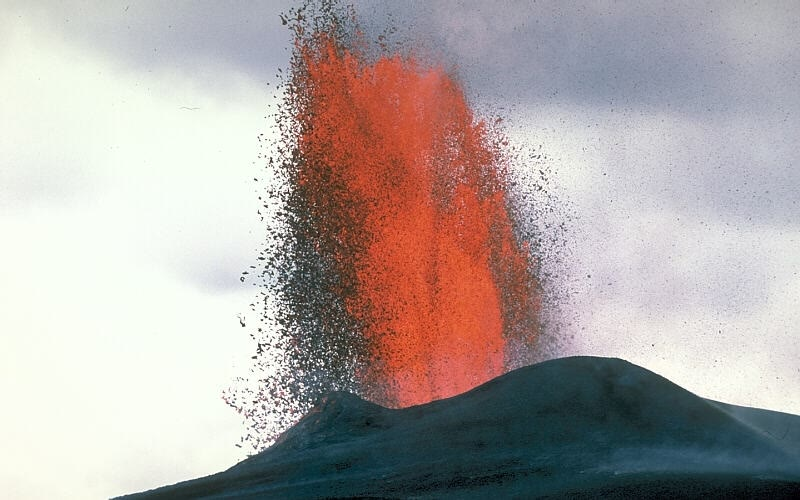
\includegraphics[height=4.3cm]{images/book4/b2-kilauea-fountain.jpg}\hfill
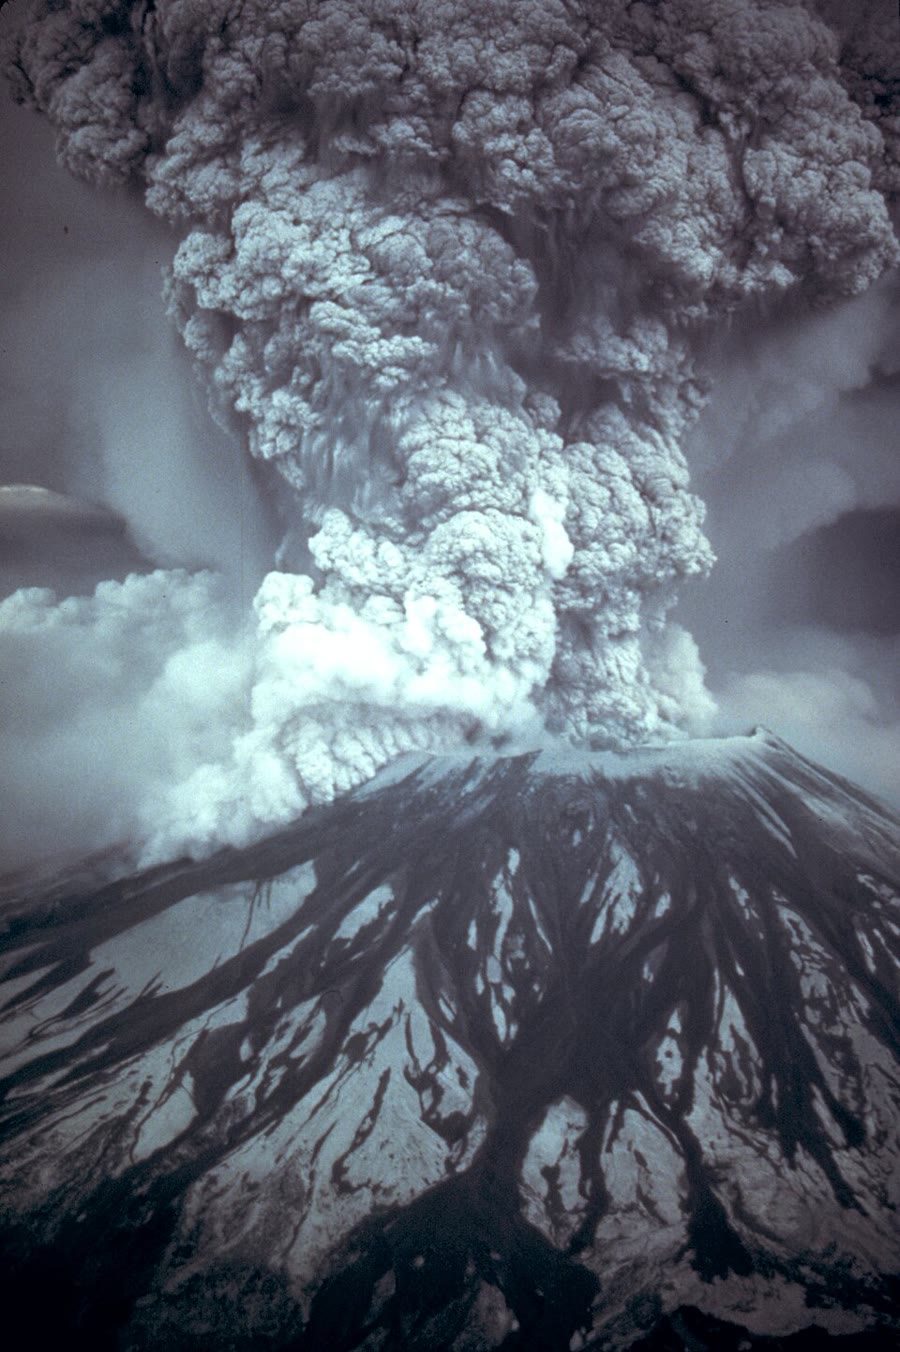
\includegraphics[height=4.3cm]{images/book4/b2-st-helens-column.jpg}\hfill
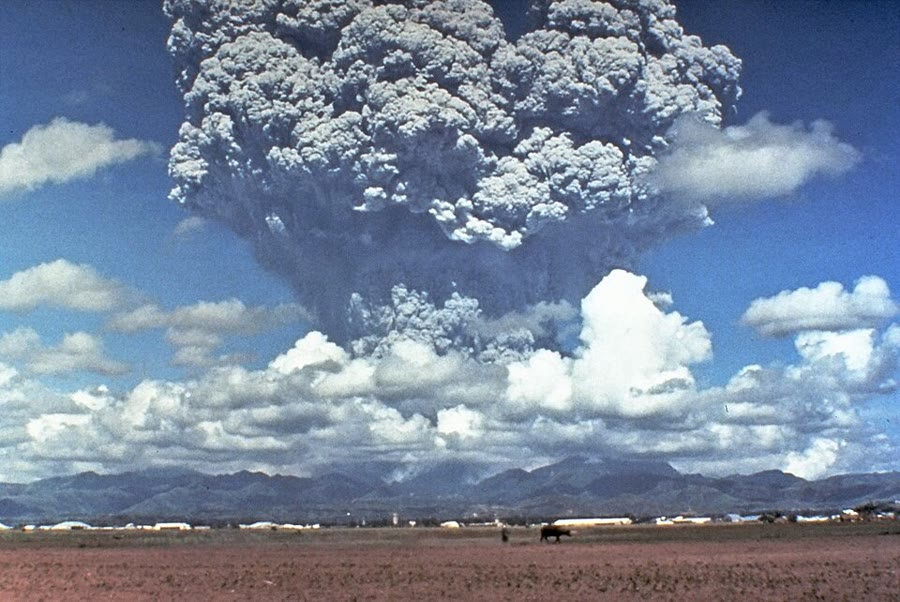
\includegraphics[height=4.3cm]{images/book4/b2-pinatubo-column.jpg}
\par\smallskip{\small Left: a Hawaiian fountain on the Pu`u~`\=O`\=o cone of Kīlauea,
October 1983 (J.\,D.~Griggs, USGS). Centre: the Plinian column of Mount St.~Helens,
18 May 1980 (Austin Post, USGS). Right: the \omterm{def:b2:eruptive-styles:column}{eruption column} of Mount Pinatubo on
12 June 1991, three days before the climactic eruption (Dave Harlow, USGS). All
three photographs are in the public domain.}
\end{omfigure}
% ledger: usgs:puuoo, usgs:msh-may18, usgs:pinatubo-1991

\section{Eruption columns}

\begin{definition}[Eruption column]\label{def:b2:eruptive-styles:column}
An \emph{eruption column}\index{eruption column} is the ascending mass of gas and
fragments above an explosive vent. It has three parts: a \emph{jet}, or
gas-thrust region, in which the mixture leaves the vent fast but denser than the
air and rises on its momentum; a \emph{convective} region, in which the mixture,
having engulfed and heated enough air to become lighter than its surroundings,
rises by buoyancy; and an \emph{umbrella} cloud, which spreads sideways at the
level where the column's density equals that of the atmosphere.
\end{definition}
% ledger: usgs:glossary-ch6, nps:styles, aubry23:fits

\begin{omfigure}
\centering
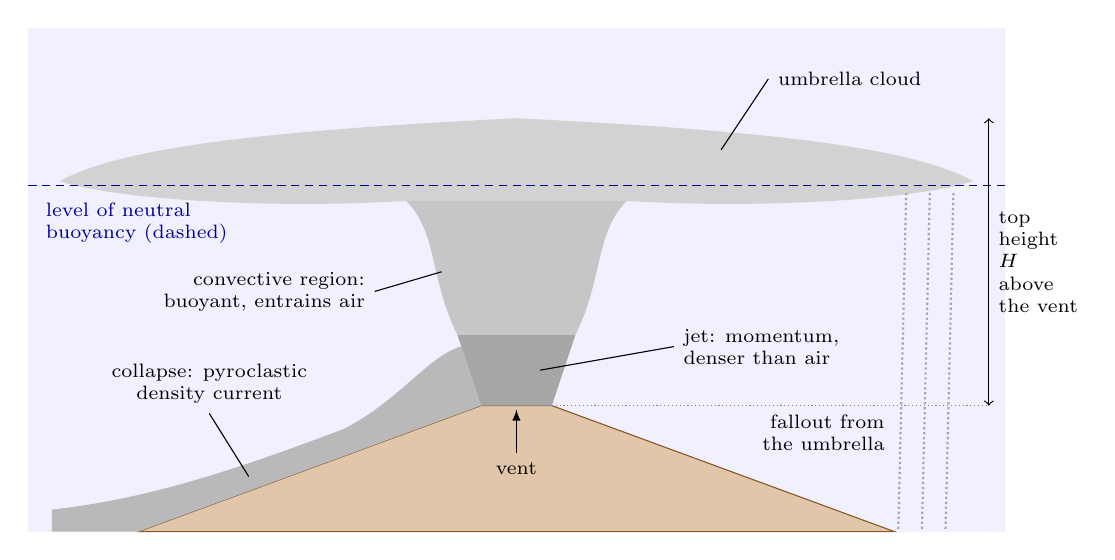
\begin{tikzpicture}[x=1cm, y=1cm, font=\scriptsize]
% atmosphere and ground
\fill[blue!6] (-6.2,0) rectangle (6.2,6.4);
% volcano
\fill[brown!45, draw=brown!70!black] (-4.8,0) -- (-0.45,1.6) -- (0.45,1.6) -- (4.8,0) -- cycle;
% collapse branch (left): a density current hugging the flank
\fill[gray!55] (-0.45,1.6) -- (-0.7,2.35) .. controls (-1.1,2.25) and (-1.5,1.65) .. (-2.2,1.3)
  .. controls (-3.4,0.85) and (-4.6,0.42) .. (-5.9,0.28) -- (-5.9,0) -- (-4.8,0) -- cycle;
% jet
\fill[gray!70] (-0.45,1.6) -- (0.45,1.6) -- (0.75,2.5) -- (-0.75,2.5) -- cycle;
% convective column
\fill[gray!45] (-0.75,2.5) .. controls (-1.1,3.2) and (-1.0,3.8) .. (-1.4,4.2)
  -- (1.4,4.2) .. controls (1.0,3.8) and (1.1,3.2) .. (0.75,2.5) -- cycle;
% umbrella
\fill[gray!35] (-1.4,4.2) .. controls (-3,4.1) and (-5,4.2) .. (-5.8,4.45)
  .. controls (-5,4.9) and (-3,5.1) .. (0,5.25) .. controls (3,5.1) and (5,4.9) .. (5.8,4.45)
  .. controls (5,4.2) and (3,4.1) .. (1.4,4.2) -- cycle;
\draw[densely dashed, blue!60!black] (-6.2,4.4) -- (6.2,4.4);
% fallout from the far end of the umbrella, down to the ground
\foreach \x in {4.95,5.25,5.55} {\draw[gray!70, densely dotted, thick] (\x,4.3) -- (\x-0.1,0.02);}
\draw[gray, densely dotted] (0.45,1.6) -- (6.0,1.6);
\draw[<->] (6.0,1.6) -- (6.0,5.25) node[midway, right, align=left] {top\\height\\$H$\\above\\the vent};
% labels
\node[anchor=north west, align=left, blue!60!black] at (-6.1,4.3) {level of neutral\\buoyancy (dashed)};
\draw (-0.95,3.3) -- (-1.8,3.05) node[left, align=right] {convective region:\\buoyant, entrains air};
\draw (0.3,2.05) -- (2.0,2.35) node[right, align=left] {jet: momentum,\\denser than air};
\draw (2.6,4.85) -- (3.2,5.75) node[right] {umbrella cloud};
\node[anchor=east, align=right] at (4.8,1.25) {fallout from\\the umbrella};
\draw (-3.4,0.7) -- (-3.9,1.5) node[above, align=center] {collapse: pyroclastic\\density current};
\draw[-latex] (0,1.0) -- (0,1.55);
\node[anchor=north] at (0,1.0) {vent};
\end{tikzpicture}
\par\smallskip{\small Anatomy of an \omterm{def:b2:eruptive-styles:column}{eruption column} (schematic, not to scale). On
the right the column rises through its three regions and the umbrella cloud
drops \omterm{def:b2:eruptive-styles:tephra}{tephra} as it spreads; on the left, part of the jet has failed to become
buoyant and collapses into a \omterm{def:b2:eruptive-styles:pdc}{pyroclastic density current}.}
\end{omfigure}

How high a column rises depends above all on how much heat it brings each
second, that is on the mass eruption rate~$Q$. Dimensional analysis gives the
form of the law.

\begin{proposition}[Height of a buoyant plume]\label{prop:b2:eruptive-styles:plume}
If the top height $H$ of a buoyant plume above a steady point source depends only
on the source's buoyancy flux $F$ (dimension $\mathrm{m^4\,s^{-3}}$) and on the
buoyancy frequency $N$ of a stably stratified atmosphere (dimension
$\mathrm{s^{-1}}$), then
\[
H = c\,F^{1/4}N^{-3/4}
\]
with $c$ a dimensionless constant. Since $F$ is proportional to the heat flux, and so
to the mass eruption rate, $H \propto Q^{1/4}$ in a given atmosphere.
\end{proposition}

\begin{proof}
Write $H = c\,F^{\alpha}N^{\beta}$. Matching lengths gives $4\alpha = 1$; matching
times gives $-3\alpha - \beta = 0$. Hence $\alpha = 1/4$ and $\beta = -3/4$, and no
other combination of $F$ and $N$ has the dimension of a length.
\end{proof}

The constant $c$ comes from how fast the plume engulfs air, which plume theory
treats with an entrainment coefficient measured in experiments; it is admitted
here. Real columns are not steady point sources in a calm atmosphere, so
volcanologists fit the law to eruptions whose height and mass eruption rate were
both measured.
% ledger: aubry23:fits

\begin{proposition}[Column height and mass eruption rate]\label{prop:b2:eruptive-styles:mastin}
For the top height $H$ above the vent in kilometres and the mass eruption rate
$Q$ in kilograms per second, the compilation of well-documented eruptions gives
\[
H = 0.304\,Q^{0.241},
\]
and a larger, independent data set of 130 events gives $H = 0.345\,Q^{0.226}$.
The scatter is large: the relative root-mean-square error on $H$ is
\qtyrange{53}{60}{\percent}.
\end{proposition}
\admitted
% ledger: aubry23:fits

Both exponents are close to the $1/4$ of plume theory. The figure below shows
the two fits and the example eruptions on which the source parameters used by
ash-forecasting centres are based. A column \qty{15}{km} high, like Mount
St.~Helens', needs \qty{e7}{kg/s}, ten thousand tonnes each second; doubling the
height needs nearly eighteen times the rate. Read the other way, a measured height gives
the rate, but only to within a factor of several, because $Q$ goes as $H^4$
(\cref{exo:b2:eruptive-styles:3}). Volcanologists express the rate by the \emph{intensity} $I =
\log_{10}Q + 3$, with $Q$ in kilograms per second.
% ledger: mastin09:examples, aubry23:fits, brown14:record

\begin{omfigure}
\centering
\begin{tikzpicture}
\begin{axis}[omrecord, width=0.82\linewidth, height=6cm, xmode=log, ymode=log,
  xmin=1e3, xmax=1e9, ymin=1, ymax=60,
  xlabel={mass eruption rate $Q$ (\unit{kg/s})}, ylabel={top height above vent (\unit{km})},
  ytick={1,2,5,10,20,50}, yticklabels={1,2,5,10,20,50},
  legend pos=north west, legend style={font=\scriptsize},
  tick label style={font=\scriptsize}, label style={font=\small}]
\addplot[very thick, black] table[x=Q, y=mastin] {figdata/out/bachelor-2-eruptions-column.dat};
\addlegendentry{$H = 0.304\,Q^{0.241}$}
\addplot[thick, red!70!black, dashed] table[x=Q, y=aubry] {figdata/out/bachelor-2-eruptions-column.dat};
\addlegendentry{$H = 0.345\,Q^{0.226}$}
\addplot[only marks, mark=*, mark size=1.8pt, blue!70!black]
  table[x=Q, y=H] {figdata/out/bachelor-2-eruptions-column-data.dat};
\addlegendentry{example eruptions}
\begin{scope}[font=\tiny, inner sep=1.5pt]
\node[anchor=north west] at (axis cs:5e3,2) {Etna 2001};
\node[anchor=south east] at (axis cs:1e5,7) {Cerro Negro 1992};
\node[anchor=north west] at (axis cs:2e5,5) {Ruapehu 1996};
\node[anchor=east] at (axis cs:1e6,10) {Fuego 1974};
\draw[gray] (axis cs:3e6,10) -- (axis cs:2e7,4.5) node[anchor=west, black] {Soufri\`ere Hills};
\draw[gray] (axis cs:4e6,11) -- (axis cs:2e7,6.5) node[anchor=west, black] {Spurr 1992};
\node[anchor=south east] at (axis cs:1e7,15) {St Helens 1980};
\node[anchor=south east, align=right] at (axis cs:1e8,25) {St Helens\\co-ignimbrite};
\end{scope}
\end{axis}
\end{tikzpicture}
\par\smallskip{\small Top height of \omterm{def:b2:eruptive-styles:column}{eruption columns} above the vent against the
mass eruption rate: the empirical fit of Mastin and others (2009), the fit of
Aubry and others (2023) to an independent data set, and the example eruptions
of the first compilation (the \omterm{def:b2:eruptive-styles:pdc}{co-ignimbrite} cloud of Mount St.~Helens rose from
\omterm{def:b2:eruptive-styles:pdc}{pyroclastic flows}, not from the vent).}
\end{omfigure}
% ledger: aubry23:fits, mastin09:examples

A column can also fail to rise. The jet leaves the vent denser than air; if it
runs out of momentum before it has engulfed enough air to become buoyant, for
instance because its gas content drops, the column collapses and the mixture
pours down the flanks as a hot, dense current. Plinian columns can collapse in
this way, and at Pinatubo the \omterm{def:b2:eruptive-styles:pdc}{pyroclastic flows} of 1991 filled valleys with
deposits as much as \qty{200}{m} thick.
% ledger: nps:styles, usgs:pinatubo-deposits

\section{Pyroclastic products}

\begin{definition}[Tephra and pyroclasts]\label{def:b2:eruptive-styles:tephra}
A \emph{pyroclast}\index{pyroclast} is a fragment produced by the explosive
fragmentation of \omterm{def:b2:magma-emplacement:magma}{magma} or of the rocks around it. \emph{Tephra}\index{tephra} is
the collective name of all pyroclasts thrown into the air, whatever their size.
By size, pyroclasts finer than \qty{2}{mm} make volcanic ash; those of
\qtyrange{2}{64}{mm} are \emph{lapilli}\index{lapilli}; those larger than
\qty{64}{mm} are blocks if they were solid when ejected and angular, and a
\emph{volcanic bomb}\index{volcanic bomb} if they were wholly or partly molten
and took a rounded or spindle shape in flight.
\end{definition}
% ledger: nps:pyroclast-sizes, usgs:glossary-ch6

\omterm{def:b2:eruptive-styles:tephra}{Tephra} falls from the umbrella cloud and the column downwind as a fall deposit
that blankets the land: thick near the vent, thinner and finer away from it. Its
thickness is mapped by \emph{isopachs}, lines of equal thickness, and, as a rule,
decreases exponentially with distance. Because the wind stretches the isopachs
into ellipses, distance is best measured by the square root of the area each
isopach encloses.
% ledger: usgs:ash-props, biass19:layer5

\begin{proposition}[Volume of an exponentially thinning deposit]\label{prop:b2:eruptive-styles:thinning}
If the thickness of a fall deposit decreases with the square root $x = \sqrt A$
of the isopach area as $T = T_0\,e^{-kx}$, its bulk volume is
\[
V = \frac{2T_0}{k^2}.
\]
Half of that volume lies beyond the isopach $x_{1/2} = 1.678/k$.
\end{proposition}

\begin{proof}
Between the isopachs of areas $A$ and $A + dA$ the deposit has volume $T\,dA$,
and $dA = 2x\,dx$. So $V = \int_0^\infty T_0e^{-kx}\,2x\,dx = 2T_0/k^2$, by
integration by parts ($\int_0^\infty xe^{-kx}dx = 1/k^2$). The volume inside $x$
is $\frac{2T_0}{k^2}[1 - (1 + kx)e^{-kx}]$, which is half the total when $(1 +
u)e^{-u} = 1/2$ with $u = kx$, that is $u = 1.678$.
\end{proof}

Real deposits thin with two or more slopes, steep near the vent and gentle far
away, because the coarse \omterm{def:b2:eruptive-styles:tephra}{lapilli} fall fast from the column and the fine ash
drifts. Each segment is fitted separately and the integral is taken piece by
piece.

\begin{method}[Volume of a fall deposit from its isopachs]\label{met:b2:eruptive-styles:volume}
Plot $\ln T$ against $\sqrt A$ for each isopach and fit a straight line to each
run of aligned points. For two segments, $T_0e^{-k_1x}$ inside the crossing point
$X$ of the two lines and the second one beyond it, the volume is
\[
V = \frac{2T_0}{k_1^2} + 2T_0e^{-k_1X}\left[\frac{k_2X + 1}{k_2^2} -
\frac{k_1X + 1}{k_1^2}\right]
\]
(\cref{exo:b2:eruptive-styles:10}). Convert the bulk volume to a dense-rock equivalent, the volume of
the same mass as bubble-free \omterm{def:b2:magma-emplacement:magma}{magma}, by $V_{\mathrm{DRE}} = V\rho_{\mathrm{deposit}}/\rho_{\mathrm{magma}}$.
\end{method}
% ledger: biass19:layer5, brown14:record

The figure below applies the method to a scoria fall erupted by Cotopaxi, in
Ecuador, about \num{1200} years ago. Two segments fit the six isopachs, with
thickness half-distances $\ln 2/k$ of \qty{1.9}{km} and \qty{5.0}{km} (the
published study, whose fit differs slightly, finds \qty{1.9}{km} and
\qty{5.3}{km}), and the volume comes out at \qty{0.29}{km^3}, as in that study. More than
\qty{40}{\percent} of it lies in the thin distal segment, which is why distal ash,
easily eroded or never mapped, matters so much to the total. Freshly fallen ash
has a bulk density of \qtyrange{500}{1500}{kg/m^3}, well below that of the
\omterm{def:b2:magma-emplacement:magma}{magma}, so the dense-rock equivalent is roughly half the bulk volume or less.
% ledger: biass19:layer5, usgs:ash-props

\begin{omfigure}
\centering
\begin{tikzpicture}
\begin{axis}[omrecord, width=0.78\linewidth, height=5.6cm, ymode=log,
  xmin=0, xmax=30, ymin=2, ymax=2000,
  xlabel={$\sqrt{\text{isopach area}}$ (\unit{km})}, ylabel={thickness (\unit{cm})},
  ytick={2,5,10,20,50,100,200,500,1000,2000}, yticklabels={2,5,10,20,50,100,200,500,1000,2000},
  legend pos=north east, legend style={font=\scriptsize},
  tick label style={font=\scriptsize}, label style={font=\small}]
\addplot[thick, black, restrict x to domain=0:12] table[x=sqrtA_km, y=seg1] {figdata/out/bachelor-2-eruptions-thin-fit.dat};
\addlegendentry{proximal segment, $k_1 = \qty{0.365}{km^{-1}}$}
\addplot[thick, red!70!black, dashed, restrict x to domain=5:30] table[x=sqrtA_km, y=seg2] {figdata/out/bachelor-2-eruptions-thin-fit.dat};
\addlegendentry{distal segment, $k_2 = \qty{0.138}{km^{-1}}$}
\addplot[only marks, mark=*, mark size=2pt, blue!70!black] table[x=sqrtA_km, y=T_cm] {figdata/out/bachelor-2-eruptions-thin-data.dat};
\addlegendentry{isopachs}
\end{axis}
\end{tikzpicture}
\par\smallskip{\small Thinning of the Layer~5 scoria fall of Cotopaxi (Ecuador),
about \num{1200} years old: isopach thicknesses from Biass, Bonadonna and
Houghton (2019) against the square root of the area each isopach encloses (the
vertical scale is logarithmic). Two exponential segments, fitted to the two
proximal and the four distal isopachs, cross at $\sqrt A = \qty{8.6}{km}$;
integrated, they give a bulk volume of \qty{0.29}{km^3}.}
\end{omfigure}
% ledger: biass19:layer5

Not all \omterm{def:b2:eruptive-styles:tephra}{tephra} falls from the sky. When a column collapses, a dome crumbles or a
lateral blast tears open the side of a volcano, the hot mixture runs along the
ground.

\begin{definition}[Pyroclastic density currents]\label{def:b2:eruptive-styles:pdc}
A \emph{pyroclastic density current}\index{pyroclastic density current} is a
ground-hugging mixture of hot gas and \omterm{def:b2:eruptive-styles:tephra}{pyroclasts} that flows downhill or outwards
because it is denser than the air. A \emph{pyroclastic flow}\index{pyroclastic
flow} is a concentrated current of rock fragments, ash and gas, typically hotter
than \qty{800}{\celsius}, that moves at tens of metres per second; a
\emph{pyroclastic surge}\index{pyroclastic surge} is a more dilute cloud of ash,
rock and gas, of several hundred degrees, that moves at the speed of a hurricane
wind. An \emph{ignimbrite}\index{ignimbrite} is the rock deposited by pyroclastic
density currents, which may be welded by its own heat.
\end{definition}
% ledger: usgs:glossary-ch6

On 18 May 1980 the collapse of the north flank of Mount St.~Helens, the largest
landslide in recorded history at about \qty{2.8}{km^3}, unroofed the \omterm{def:b2:magma-emplacement:magma}{magma} and
released a lateral blast that crossed about \qty{600}{km^2} at up to
\qty{480}{km/h}; \omterm{def:b2:eruptive-styles:pdc}{pyroclastic flows} of at least \qty{700}{\celsius} then reached
\qty{8}{km} from the crater. Pinatubo's flows of 1991 were still as hot as
\qty{500}{\celsius} inside five years later.
% ledger: usgs:msh-may18, usgs:msh-flows, usgs:msh-reach, usgs:pinatubo-deposits

\begin{definition}[Lahar]\label{def:b2:eruptive-styles:lahar}
A \emph{lahar}\index{lahar} is a fast-moving mixture of water and volcanic debris
that flows down a river valley, with the consistency of anything from muddy water
to wet concrete. Lahars form when pyroclastic currents melt snow and ice, when
heavy rain falls on loose volcanic deposits, when a lake dammed by volcanic
deposits breaks out, or from a debris avalanche.
\end{definition}
% ledger: usgs:glossary-ch6

\omterm{def:b2:eruptive-styles:lahar}{Lahars} outlast eruptions. Around Pinatubo, monsoon and typhoon rains turned the
ash of 1991 into \omterm{def:b2:eruptive-styles:lahar}{lahars} for years, and they caused more destruction than the
eruption itself.
% ledger: usgs:pinatubo-lahars

\begin{definition}[Caldera]\label{def:b2:eruptive-styles:caldera}
A \emph{caldera}\index{caldera} is a large basin-shaped volcanic depression,
\qtyrange{2}{50}{km} across and much wider than any vent within it, formed by
the collapse of the ground into a shallow \omterm{def:b2:magma-emplacement:magma}{magma} reservoir that an eruption has
partly emptied.
\end{definition}
% ledger: usgs:glossary-ch6

Pinatubo's and Novarupta's \omterm{def:b2:eruptive-styles:caldera}{calderas} are both about \qty{2.5}{km} across, at the
small end of the range. A \omterm{def:b2:eruptive-styles:caldera}{caldera} differs from a crater, which is smaller and excavated by explosions.
% ledger: usgs:pinatubo-1991, nps:styles, usgs:glossary-ch6

\section{Measuring and counting eruptions}

\begin{definition}[Volcanic Explosivity Index]\label{def:b2:eruptive-styles:vei}
The \emph{Volcanic Explosivity Index}\index{Volcanic Explosivity Index} (VEI) is
an integer from 0 to 8 that measures the size of an eruption, chiefly by the
bulk volume of its \omterm{def:b2:eruptive-styles:tephra}{tephra}: VEI~0 for less than \qty{e4}{m^3}, VEI~1 up to
\qty{e6}{m^3}, then one step for every factor of ten, up to VEI~8 beyond
\qty{e12}{m^3}, \qty{1000}{km^3}. Column height and descriptions of the eruption
are used when the volume is not known. A non-explosive eruption has VEI~0,
whatever the volume of its lava.
\end{definition}
% ledger: usgs:vei-criteria, usgs:msh-comparisons

\begin{table}[ht]
\centering
\small
\begin{tabular}{llll}
\hline
VEI & bulk \omterm{def:b2:eruptive-styles:tephra}{tephra} volume (\unit{m^3}) & column height (\unit{km}) & usual style \\
\hline
0 & $< 10^{4}$ & $< 0.1$ & Hawaiian \\
1 & $10^{4}$--$10^{6}$ & 0.1--1 & Hawaiian, Strombolian \\
2 & $10^{6}$--$10^{7}$ & 1--5 & Strombolian, Vulcanian \\
3 & $10^{7}$--$10^{8}$ & 3--15 & Vulcanian \\
4 & $10^{8}$--$10^{9}$ & 10--25 & Vulcanian, Plinian \\
5 & $10^{9}$--$10^{10}$ & $> 25$ & Plinian \\
6 & $10^{10}$--$10^{11}$ & $> 25$ & Plinian \\
7 & $10^{11}$--$10^{12}$ & $> 25$ & Plinian \\
8 & $> 10^{12}$ & $> 25$ & Plinian \\
\hline
\end{tabular}
\caption{Criteria of the \omterm{def:b2:eruptive-styles:vei}{Volcanic Explosivity Index} (after Newhall and Self, 1982).}
\label{tab:b2:eruptive-styles:vei}
\end{table}
% ledger: usgs:vei-criteria

The index is logarithmic like an earthquake magnitude, but coarser. Mount
St.~Helens in 1980, with \qty{1.3}{km^3} of ash, rated VEI~5 ``but just barely'';
Pinatubo in 1991 rated VEI~6; Tambora in 1815, which ejected thirty to eighty
times more ash than Mount St.~Helens, rated VEI~7, the largest \omterm{def:b2:eruptive-styles:regimes}{explosive eruption}
of historic times. For quantitative work volcanologists prefer the
\emph{magnitude} $M = \log_{10}m - 7$, with $m$ the erupted mass in kilograms, which
avoids the bulk density of the deposit, and the intensity defined above for the
rate.
% ledger: usgs:msh-1980-ash, usgs:msh-comparisons, data:b4-gvp-eruptions, brown14:record

Small eruptions are frequent and large ones rare. The global catalogue of
Holocene eruptions makes the relation quantitative, once one allows for its
gaps: an eruption is in the catalogue only if someone recorded it or found its
deposit, and small eruptions far from observers, or more than a few centuries
old, were often missed. The record of large eruptions is complete for longer than
that of small ones. In the left panel of the figure below, the eruptions of each
size recorded since 1500 accumulate with time; a complete record at a constant
rate would follow the diagonal. Eruptions of VEI~3 or more bunch into the last
century, because most of the earlier ones were never recorded; the VEI~6 record
is close to the diagonal.
% ledger: data:b4-gvp-eruptions, brown14:record

\begin{dated}{2026}
The catalogue of the Global Volcanism Program lists \num{7747} confirmed Holocene
eruptions with a VEI. Counted from the start of a window to the end of 2024, there
were 399 eruptions of VEI~3 or more since 1950, 95 of VEI~4 or more since 1900,
22 of VEI~5 or more since 1800, and 8 of VEI~6 or more since 1500 (the most
recent, Pinatubo in 1991). Only two eruptions of VEI~7 are recorded since the year
1000: Rinjani in 1257 and Tambora, whose eruption began in 1812 and culminated in
1815.
\end{dated}
% ledger: data:b4-gvp-eruptions, usgs:msh-comparisons

\begin{proposition}[Frequency--size law of eruptions]\label{prop:b2:eruptive-styles:frequency}
Let $\lambda_v$ be the mean number of eruptions of VEI $\ge v$ per year on Earth,
each estimated over a window in which its record is close to complete (from 1950
for $v = 3$, 1900 for $v = 4$, 1800 for $v = 5$, 1500 for $v = 6$). Then, by least
squares,
\[
\log_{10}\lambda_v = 3.28 - 0.85\,v .
\]
Each step of VEI is about seven times rarer than the one below it.
\end{proposition}
% ledger: data:b4-gvp-eruptions

The law is empirical, a fit to four points, and its exponent depends on the
windows chosen; it predicts one eruption of VEI~7 or more every \num{470} years,
close to the two in the last thousand years that were not used to fit it. Since
the eruptions are nearly independent of one another, they behave as a Poisson
process, and the probability of at least one eruption of VEI $\ge v$ in $t$ years
is $1 - e^{-\lambda_vt}$ (weekend problem).
% ledger: data:b4-gvp-eruptions

\begin{omfigure}
\centering
\begin{tikzpicture}
\begin{axis}[omrecord, name=cum, width=0.47\linewidth, height=5.6cm,
  xmin=1500, xmax=2024, ymin=0, ymax=1,
  xlabel={year}, ylabel={fraction recorded since 1500},
  xtick={1500,1600,1700,1800,1900,2000}, x tick label style={/pgf/number format/1000 sep={}},
  legend pos=north west, legend style={font=\tiny},
  tick label style={font=\scriptsize}, label style={font=\small}]
\addplot[thick, gray, densely dotted, domain=1500:2024, samples=2] {(x - 1500)/524};
\addlegendentry{constant rate}
\addplot[thick, blue!70!black] table[x=year, y=f3] {figdata/out/bachelor-2-eruptions-vei-cumul.dat};
\addlegendentry{VEI $\ge 3$}
\addplot[thick, black, dashed] table[x=year, y=f4] {figdata/out/bachelor-2-eruptions-vei-cumul.dat};
\addlegendentry{VEI $\ge 4$}
\addplot[thick, orange!80!black, dashdotted] table[x=year, y=f5] {figdata/out/bachelor-2-eruptions-vei-cumul.dat};
\addlegendentry{VEI $\ge 5$}
\addplot[thick, red!70!black, const plot] table[x=year, y=f6] {figdata/out/bachelor-2-eruptions-vei-cumul.dat};
\addlegendentry{VEI $\ge 6$}
\end{axis}
\begin{axis}[omrecord, at={(cum.east)}, anchor=west, xshift=1.9cm,
  width=0.47\linewidth, height=5.6cm, ymode=log,
  xmin=2.5, xmax=7.5, ymin=1e-3, ymax=20,
  xlabel={VEI $v$}, ylabel={eruptions of VEI $\ge v$ per year},
  xtick={3,4,5,6,7},
  tick label style={font=\scriptsize}, label style={font=\small}]
\addplot[thick, black] table[x=vei, y=rate] {figdata/out/bachelor-2-eruptions-vei-fit.dat};
\addplot[only marks, mark=*, mark size=2pt, blue!70!black] table[x=vei, y=rate] {figdata/out/bachelor-2-eruptions-vei-rate.dat};
\addplot[only marks, mark=o, mark size=2.4pt, red!70!black] table[x=vei, y=rate] {figdata/out/bachelor-2-eruptions-vei-rate7.dat};
\node[font=\tiny, anchor=south west] at (axis cs:3.05,6) {since 1950};
\node[font=\tiny, anchor=south west] at (axis cs:4.05,0.8) {since 1900};
\node[font=\tiny, anchor=south west] at (axis cs:5.05,0.1) {since 1800};
\node[font=\tiny, anchor=south west] at (axis cs:6.05,0.016) {since 1500};
\node[font=\tiny, anchor=east, red!70!black] at (axis cs:6.85,0.00195) {since 1000};
\end{axis}
\end{tikzpicture}
\par\smallskip{\small Left: completeness of the global record. For each size,
the fraction of the eruptions recorded between 1500 and 2024 that had already
occurred by a given year; a complete record at a constant rate would follow the
dotted diagonal. Right: annual rate of eruptions of VEI $\ge v$, each counted over
its own window, and the least-squares line of
\cref{prop:b2:eruptive-styles:frequency}; the open circle, VEI $\ge 7$ since the year
1000, was not used in the fit. Data: Global Volcanism Program, Volcanoes of the
World.}
\end{omfigure}
% ledger: data:b4-gvp-eruptions

\section{Watching volcanoes}

\omterm{def:b2:magma-emplacement:magma}{Magma} does not reach the surface unannounced. It must break rock to open its
path, it pushes the ground up as it accumulates, it releases gas as the pressure
on it falls, and it heats the ground. Volcano observatories monitor all four.

\emph{Seismicity.} \omterm{def:b2:magma-emplacement:magma}{Magma} moving through the crust breaks rock and sets off swarms
of small earthquakes. Before 18 May 1980 Mount St.~Helens produced more than
\num{10000} of them in two months; Pinatubo produced thousands between April and
June 1991, from \omterm{def:b2:magma-emplacement:magma}{magma} rising from more than \qty{32}{km} below. The magnitudes
and the seismic moments of the Year 1 volume apply unchanged; what differs is the
sources, opening cracks and resonating fluid-filled conduits as well as faults.
% ledger: usgs:msh-lead-up, usgs:pinatubo-deposits

\emph{Deformation.} A reservoir that fills inflates and lifts the ground above
it. Levelling, tiltmeters and satellite positioning measure the uplift; radar interferometry from satellites maps it over whole
volcanoes, a technique the Year 3 volume of this series explains. The simplest
model treats the reservoir as a small sphere.

\begin{proposition}[Mogi source]\label{prop:b2:eruptive-styles:mogi}
A small spherical source at depth $z_0$ in a homogeneous elastic half-space
with Poisson's ratio $\nu$, whose volume changes by $\Delta V$, a
\emph{Mogi source}\index{Mogi source}, lifts the surface at horizontal distance $r$
by
\[
u_z(r) = \frac{(1 - \nu)\,\Delta V}{\pi}\,\frac{z_0}{(r^2 + z_0^2)^{3/2}} .
\]
\end{proposition}
\admitted
% ledger: dmodels:mogi

The uplift is largest above the source, $u_z(0) = (1 - \nu)\Delta V/(\pi z_0^2)$, and
falls to half that at $r = z_0\sqrt{2^{2/3} - 1} = 0.766\,z_0$: the width of the
bulge gives the depth of the source, and its height then gives the volume
change. Because only $\Delta V$ enters, the pressure in the reservoir and its size
cannot be separated, so volume changes, not pressures, are what geodesists
report. The formula is the first term of an exact solution for a sphere of radius
$a$; the correction is \qty{12}{\percent} when $a = z_0/2$ and \qty{3}{\percent}
when $a = z_0/3$.
% ledger: dmodels:mogi

\begin{omfigure}
\centering
\begin{tikzpicture}
\begin{axis}[omrecord, width=0.78\linewidth, height=5.2cm,
  xmin=-12, xmax=12, ymin=0, ymax=65,
  xlabel={horizontal distance from the source (\unit{km})}, ylabel={uplift (\unit{mm})},
  legend pos=north east, legend style={font=\scriptsize},
  tick label style={font=\scriptsize}, label style={font=\small}]
\addplot[very thick, black] table[x=r_km, y=z2] {figdata/out/bachelor-2-eruptions-mogi.dat};
\addlegendentry{source at \qty{2}{km}}
\addplot[very thick, red!70!black, dashed] table[x=r_km, y=z4] {figdata/out/bachelor-2-eruptions-mogi.dat};
\addlegendentry{source at \qty{4}{km}}
\draw[<->, thin] (axis cs:-1.532,29.8) -- (axis cs:1.532,29.8) node[midway, below, font=\tiny] {$2\times 0.766\,z_0$};
\end{axis}
\end{tikzpicture}
\par\smallskip{\small Surface uplift above a \omterm{prop:b2:eruptive-styles:mogi}{Mogi source} whose volume grows by
\qty{e6}{m^3} ($\nu = 0.25$), at two depths. Twice as deep, the bulge is four
times lower and twice as wide; the arrow marks the full width at half height of
the shallow one.}
\end{omfigure}
% ledger: dmodels:mogi

\emph{Gas and heat.} As \omterm{def:b2:magma-emplacement:magma}{magma} rises and degasses, the flux of sulfur dioxide at the
surface grows, and it is measured from the ground, from aircraft and from
satellites; Pinatubo emitted many thousand tonnes of it in the weeks before its eruption.
The heat of shallow \omterm{def:b2:magma-emplacement:magma}{magma} shows in thermal images of the ground and the vent.
% ledger: usgs:pinatubo-deposits

From these data an observatory sets an alert level. In the United States the
ground-based Volcano Alert Level, in use since 2006, has four steps, NORMAL,
ADVISORY, WATCH and WARNING, and a parallel Aviation Color Code from GREEN to RED
warns aircraft of ash. There are no fixed thresholds: each change is decided by
the observatory's scientists from all the monitoring data, the volcano's past
behaviour and what is known of the processes under way. Forecasting remains
probabilistic: when an eruption will start and how large it will be are hard to
foresee. At Pinatubo, the forecast of 1991 allowed the people living near the
volcano to move away in time and saved at least \num{5000} lives. How such forecasts
enter decisions about hazard and risk belongs to \cref{ch:b2:geological-hazards}.
% ledger: hvo:alert-levels, usgs:pinatubo-1991

\begin{inthefield}[At a volcano observatory]
\begin{minipage}[t]{0.6\linewidth}\vspace{0pt}
An observatory watches its volcanoes around the clock. Seismometers on the flanks
send their signals by radio to screens where duty scientists look for swarms,
for tremor, the continuous shaking of fluid moving in a conduit, and for changes
in the depth of the events. Positioning stations and tiltmeters record the
inflation of the ground, cameras the vent, gas spectrometers the flux of sulfur
dioxide in the plume. When a signal departs from the volcano's background, the
scientists compare it with earlier episodes, meet, and decide whether the alert
level should change; the notice they issue states what is observed and what may
follow, without overstating either.
\end{minipage}\hfill
\begin{minipage}[t]{0.36\linewidth}\vspace{0pt}
\centering
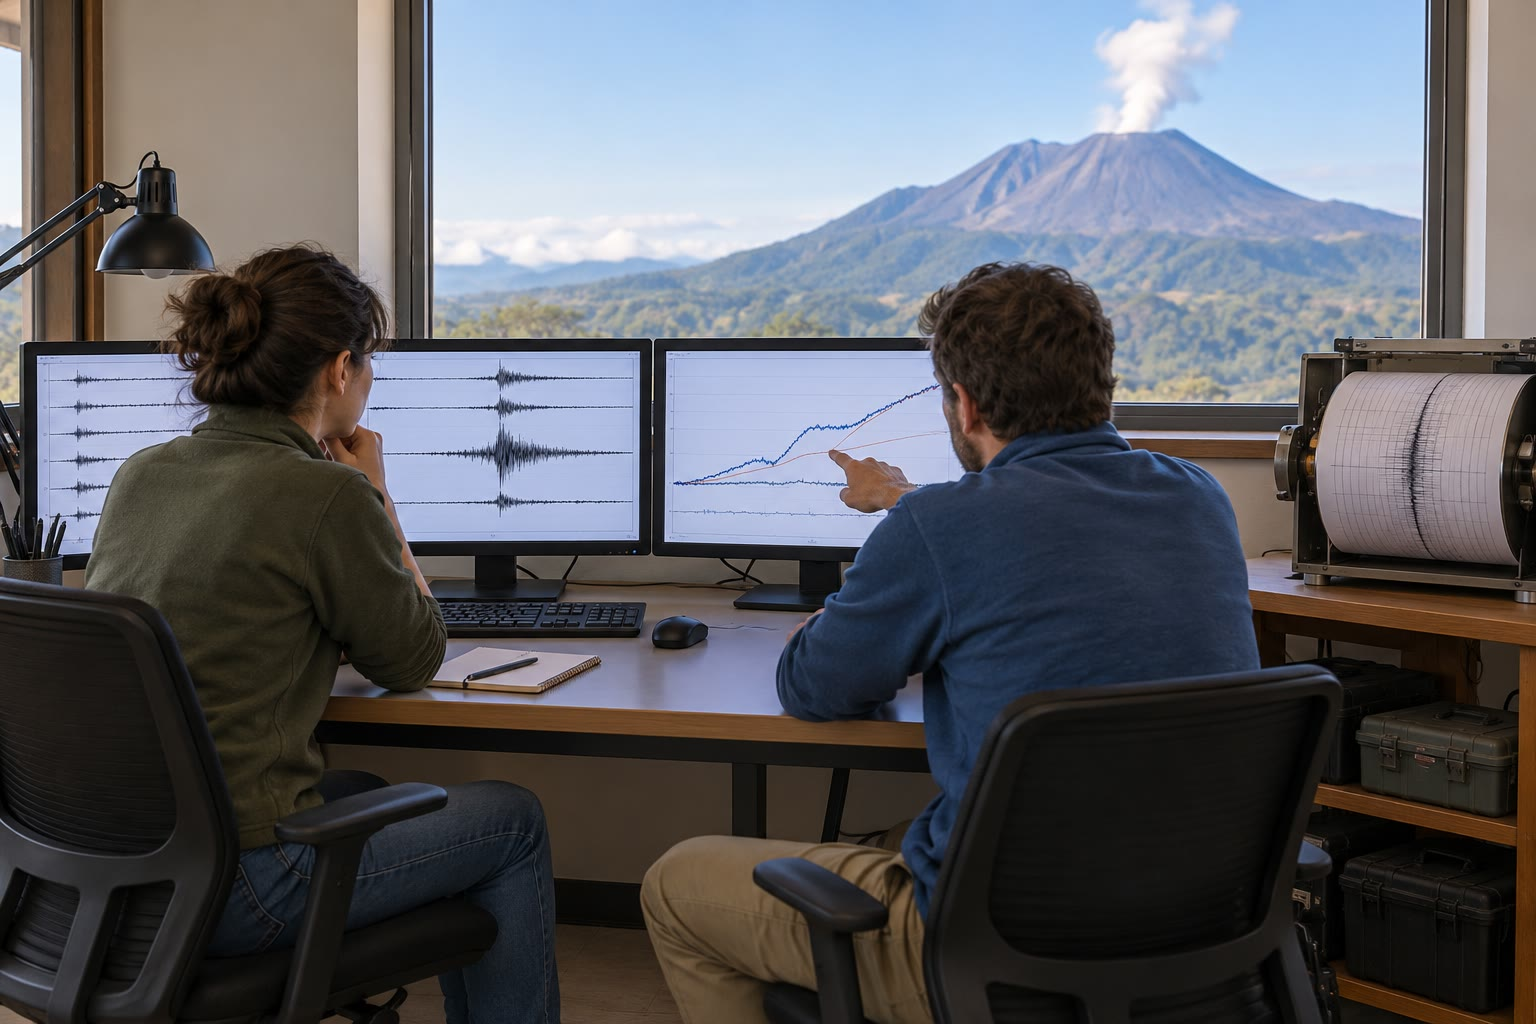
\includegraphics[width=\linewidth]{images/book4/ai/b2-volcano-observatory.jpg}
\par\smallskip{\scriptsize Scientists reviewing seismic records in a volcano
observatory (AI-generated illustration).}
\end{minipage}
\end{inthefield}
% ledger: hvo:alert-levels

\section{Exercises}

\begin{exercise}[$\star$]\label{exo:b2:eruptive-styles:1}
Give the VEI indicated by the bulk volume of \omterm{def:b2:eruptive-styles:tephra}{tephra} alone for: (a) the ash of
Mount St.~Helens, 18 May 1980, \qty{1.3}{km^3}; (b) the Layer~5 fall of Cotopaxi,
\qty{0.29}{km^3}; (c) a small eruption of \qty{2e6}{m^3}. (d) The material
ejected by Pinatubo in 1991 is given as ``more than \qty{5}{km^3}'', yet the
eruption is rated VEI~6. What bulk volume does that rating imply at least?
\end{exercise}
% ledger: usgs:vei-criteria, usgs:msh-1980-ash, biass19:layer5, usgs:pinatubo-1991

\begin{exercise}[$\star$]\label{exo:b2:eruptive-styles:2}
Name each \omterm{def:b2:eruptive-styles:tephra}{pyroclast}: (a) a glass shard \qty{0.5}{mm} long; (b) a pumice
fragment \qty{3}{cm} across; (c) an angular piece of old lava \qty{20}{cm}
across; (d) a spindle-shaped clot \qty{8}{cm} long with twisted ends.
\end{exercise}
% ledger: nps:pyroclast-sizes

\begin{exercise}[$\star$]\label{exo:b2:eruptive-styles:3}
With $H = 0.304\,Q^{0.241}$ ($H$ in kilometres above the vent, $Q$ in
\unit{kg/s}): (a) compute $H$ for $Q = \qty{e6}{kg/s}$ and \qty{e8}{kg/s};
(b) compute the mass eruption rate implied by a column \qty{35}{km} high, and its
intensity $I = \log_{10}Q + 3$; (c) by what factor does $Q$ change if the measured
height is \qty{20}{\percent} too high?
\end{exercise}
% ledger: aubry23:fits, brown14:record

\begin{exercise}[$\star$]\label{exo:b2:eruptive-styles:4}
The Layer~5 fall of Cotopaxi has a bulk volume of \qty{0.29}{km^3}. Taking a
bulk density of \qty{1000}{kg/m^3} for the deposit and \qty{2500}{kg/m^3} for the
\omterm{def:b2:magma-emplacement:magma}{magma}, compute its dense-rock equivalent volume, its mass and its magnitude
$M = \log_{10}m - 7$.
\end{exercise}
% ledger: biass19:layer5, brown14:record

\begin{exercise}[$\star\star$]\label{exo:b2:eruptive-styles:5}
A fall deposit is \qty{40}{cm} thick on the isopach of $\sqrt A = \qty{5}{km}$
and \qty{10}{cm} on that of $\sqrt A = \qty{15}{km}$, and thins as a single
exponential. Compute $k$, $T_0$, the thickness half-distance $\ln 2/k$, the bulk
volume and the VEI.
\end{exercise}

\begin{exercise}[$\star\star$]\label{exo:b2:eruptive-styles:6}
(a) Show that the volume inside the isopach $x = \sqrt A$ of a deposit thinning
as $T_0e^{-kx}$ is $\frac{2T_0}{k^2}[1 - (1 + kx)e^{-kx}]$. (b) Solve $(1 + u)e^{-u} =
1/2$ to three significant figures by repeated substitution or bisection. (c) For
the deposit of \cref{exo:b2:eruptive-styles:5}, beyond which isopach does half the volume lie? Compare
with the distance from the vent of the outermost isopach that was mapped.
\end{exercise}

\begin{exercise}[$\star\star$]\label{exo:b2:eruptive-styles:7}
A rhyolitic \omterm{def:b2:magma-emplacement:magma}{magma} at \qty{850}{\celsius} (\qty{1123}{K}) contains
\qty{5.0}{\percent} of water, with solubility $s = 0.444$ per cent per
$\sqrt{\unit{MPa}}$; its melt has a density of \qty{2300}{kg/m^3}. (a) Compute its
saturation pressure, and the depth at which it is reached for a pressure
gradient of \qty{0.025}{MPa/m}. (b) Compute the gas volume fraction at
\qty{10}{MPa} if the gas stays in the \omterm{def:b2:magma-emplacement:magma}{magma} ($R = \qty{8.314}{J/(mol.K)}$, $M =
\qty{0.018015}{kg/mol}$). (c) Why do basaltic \omterm{def:b2:magma-emplacement:magma}{magmas} fragment so much less
often, although at \qty{1}{MPa} a closed-system basalt with \qty{1}{\percent} of
water would be \qty{92}{\percent} gas?
\end{exercise}
% ledger: moore98:h2o, cassidy18:fragmentation, cassidy18:ascent

\begin{exercise}[$\star\star$]\label{exo:b2:eruptive-styles:8}
(a) A \omterm{prop:b2:eruptive-styles:mogi}{Mogi source} at \qty{5}{km} depth grows by \qty{e7}{m^3}. Compute the
uplift above it ($\nu = 0.25$). (b) Another bulge falls to half its maximum
\qty{3.8}{km} from its centre: how deep is its source? (c) What fraction of the
maximum uplift does a station see at a horizontal distance equal to the source
depth?
\end{exercise}
% ledger: dmodels:mogi

\begin{exercise}[$\star\star$]\label{exo:b2:eruptive-styles:9}
A Vulcanian explosion throws blocks out of a crater. Neglecting air resistance
and the height of the crater rim, compute the greatest range of a block launched
at \qty{100}{m/s}, then at \qty{200}{m/s} ($g = \qty{9.81}{m/s^2}$). Does air
resistance make these ranges an upper or a lower bound? Why does a zone of
ballistic hazard around a vent scale as the square of the launch speed?
\end{exercise}

\begin{exercise}[$\star\star\star$]\label{exo:b2:eruptive-styles:10}
(a) Derive the volume of a deposit with two exponential segments given in the
method box, assuming the thickness is continuous where the lines cross. (b) For
the Layer~5 fall of Cotopaxi, the fitted segments are $T = \qty{1285}{cm}\times
e^{-0.365x}$ and a distal segment of slope $k_2 = \qty{0.138}{km^{-1}}$, crossing at
$X = \qty{8.56}{km}$. Compute the volume, and the share of it beyond the crossing
point.
\end{exercise}
% ledger: biass19:layer5

\begin{exercise}[$\star\star\star$]\label{exo:b2:eruptive-styles:11}
(a) Using \cref{prop:b2:eruptive-styles:plume}, by what factor does the height of a
column rise when the eruption rate is multiplied by 100? Compare with the
empirical exponents $0.241$ and $0.226$. (b) In which way does a more strongly
stratified atmosphere change the height, and by how much if $N$ grows by
\qty{20}{\percent}? (c) Give two reasons why measured exponents may fall below
$1/4$.
\end{exercise}
% ledger: aubry23:fits

\begin{exercise}[$\star\star\star$]\label{exo:b2:eruptive-styles:12}
The global catalogue lists 132 eruptions of VEI~4 or more that began between 1500
and 1899, and 95 between 1900 and 2024. (a) Compute the rate per century in each
period. (b) If the rate since 1900 is the true one, what fraction of the earlier
eruptions was recorded? (c) A study of large eruptions finds 21 eruptions of
magnitude 4 to 4.9 per century between 1500 and 1900 and 56 since 1900; compare.
(d) Why does this fraction depend on the size of the eruptions?
\end{exercise}
% ledger: data:b4-gvp-eruptions, brown14:record

\section{Problem: Reading a Plinian deposit}

\begin{problem}[{Weekend problem --- from the isopachs of a pumice fall to the size
of its eruption, the height of its column, and how often such eruptions
happen}]
\label{pb:b2:eruptive-styles:1}
An imaginary volcano has left a pumice fall from a single Plinian phase that
lasted \qty{10}{hours}. Its isopachs, after the wind's elongation is removed by
using the square root of their areas, are:
\begin{center}
\small
\begin{tabular}{lccccc}
\hline
$\sqrt A$ (\unit{km}) & 10 & 20 & 40 & 80 & 120 \\
thickness $T$ (\unit{cm}) & 200 & 100 & 48 & 14 & 4.0 \\
\hline
\end{tabular}
\end{center}
Data: bulk density of the deposit \qty{900}{kg/m^3}; density of the \omterm{def:b2:magma-emplacement:magma}{magma}
\qty{2400}{kg/m^3}; column height measured from the largest clasts,
\qty{31}{km} above the vent; tropopause at \qty{16}{km}. Use $H =
0.304\,Q^{0.241}$ and $H = 0.345\,Q^{0.226}$ ($H$ in kilometres, $Q$ in
\unit{kg/s}).

\medskip\noindent\textbf{Part I --- The deposit.}
\begin{enumerate}
\item Compute $\ln T$ for each isopach and show that the points fall on two
straight segments when plotted against $\sqrt A$. Where is the break?
\item Compute the slope $k_1$ and the intercept $T_0$ of the proximal segment
through the first two isopachs.
\item The least-squares line through the three distal isopachs is $T =
\qty{167}{cm}\times e^{-0.0311\sqrt A}$. Check that it passes within
\qty{5}{\percent} of each of them.
\item Compute the value of $\sqrt A$ at which the two lines cross.
\item Compute the thickness half-distances $\ln 2/k$ of the two segments.
\item Compute the volume the deposit would have if it thinned with the proximal
slope everywhere.
\item Compute the bulk volume with the two segments, and the share contributed by
the correction for the gentler distal segment.
\item By what factor would the volume be underestimated if only the proximal
deposit had been mapped? Why is that a real risk for old deposits?
\end{enumerate}

\noindent\textbf{Part II --- The size of the eruption.}
\begin{enumerate}[resume]
\item Give the VEI of the eruption.
\item Compute the dense-rock equivalent volume.
\item Compute the erupted mass.
\item Compute the magnitude $M = \log_{10}m - 7$.
\item How many times larger than the ash fall of Mount St.~Helens in 1980,
\qty{1.3}{km^3}, is this deposit?
\item What column height does the VEI table associate with this eruption, and
which style?
\end{enumerate}

\noindent\textbf{Part III --- The column.}
\begin{enumerate}[resume]
\item Compute the mean mass eruption rate over the Plinian phase, and its
intensity $I = \log_{10}Q + 3$.
\item Compute the column height predicted by the first empirical law.
\item Same with the second law.
\item Compare with the \qty{31}{km} measured from the clasts, given the scatter
of the laws.
\item What mass eruption rate would \qty{31}{km} imply by the first law? By what
factor does it differ from that of question~15, and what might explain it?
\item Did the column inject gas into the stratosphere? What could follow for the
climate, and what would be the key gas?
\end{enumerate}

\noindent\textbf{Part IV --- How often?}
\begin{enumerate}[resume]
\item From the counts of the catalogue (399 eruptions of VEI $\ge 3$ from 1950 to
2024, 95 of VEI $\ge 4$ from 1900, 22 of VEI $\ge 5$ from 1800, 8 of VEI $\ge 6$ from
1500, all windows ending in 2024 inclusive), compute the four annual rates and
their logarithms.
\item Check that the line $\log_{10}\lambda_v = 3.28 - 0.85\,v$ passes within
\qty{10}{\percent} of each rate.
\item Why does each window start further back for larger eruptions?
\item From the line, compute the rate of eruptions of VEI $\ge 5$, their mean
return period, and the probability of at least one in the next 10 years.
\item From the line, compute the rate of eruptions of VEI $\ge 7$ and compare it
with the two recorded since the year 1000.
\item From the line, compute the rate of eruptions of VEI $\ge 6$ and the
probability, in per cent, of at least one somewhere on Earth in the next 100
years, the key number of this problem. What assumption does it rest on?
\end{enumerate}
\end{problem}
